\section*{Run over more than 50 epochs with varied batch
size}

Test report

by E. Marquer, 2018/06/25, Synalp and Université de Lorraine

\subsection{Abstract}

The test runs are for two parallel experiments:
\begin{itemize}
\item test which of 2 and 3
batches are the most interesting
\item test the impact of layer by layer
training (with an intuitive algorithm developed out of work-time)
\end{itemize}

The test is composed of 4 runs on grele, with:
\begin{itemize}
\item bptt 200/2, batch-size
2
\item bptt 200/3, batch-size 3
\item bptt 200/2, batch-size 2, layer by layer
training,
\item bptt 200/2, batch-size 2, layer by layer training, 20 epochs
of individual training for each layer, 10 epochs of common fine-tuning
for already trained layers (see below the explanation of this algorithm)
\end{itemize}

\subsubsection{Shared parameters}

\begin{longtable}[]{@{}ll@{}}
\hline
parameter & value\tabularnewline
\hline
\endhead
corpus & enwik8reduced\tabularnewline
history\_strategy & last\tabularnewline
max\_history & 25\tabularnewline
lr & 1e-3\tabularnewline
weight\_decay & 1.2e-6\tabularnewline
epochs & 1500\tabularnewline
valid\_len & 500,000\tabularnewline
log\_interval & 500\tabularnewline
save\_interval & 500\tabularnewline
memory\_interval & 100\tabularnewline
hidden\_size & 460\tabularnewline
embed\_size & 400\tabularnewline
growth\_factor & 5\tabularnewline
rnn\_type & RNN\tabularnewline
reset\_hidden & False\tabularnewline
reset\_growth & True\tabularnewline
cuda\_on & True\tabularnewline
\hline
\end{longtable}

\subsubsection{Model keys and
specificities}

When noting is specified, all models have:

\begin{itemize}
\item
  2 batches, and a sequence length of 200/2
\item
  1 RNN layer per MSNN layer
\end{itemize}

\begin{longtable}[]{@{}ll@{}}
\hline
\begin{minipage}[b]{0.08\columnwidth}\raggedright\strut
Model\strut
\end{minipage} & \begin{minipage}[b]{0.86\columnwidth}\raggedright\strut
Specificity\strut
\end{minipage}\tabularnewline
\hline
\endhead
\begin{minipage}[t]{0.08\columnwidth}\raggedright\strut
b2\strut
\end{minipage} & \begin{minipage}[t]{0.86\columnwidth}\raggedright\strut
classical model, comparison basis\strut
\end{minipage}\tabularnewline
\begin{minipage}[t]{0.08\columnwidth}\raggedright\strut
b3\strut
\end{minipage} & \begin{minipage}[t]{0.86\columnwidth}\raggedright\strut
3 batches, sequence length of 200/3\strut
\end{minipage}\tabularnewline
\begin{minipage}[t]{0.08\columnwidth}\raggedright\strut
s\strut
\end{minipage} & \begin{minipage}[t]{0.86\columnwidth}\raggedright\strut
``scheduled(10,10)'': use layer by layer training; 10 epochs for
individual training, 10 epochs for intermediary fine-tuning\strut
\end{minipage}\tabularnewline
\begin{minipage}[t]{0.08\columnwidth}\raggedright\strut
s-a20-l10\strut
\end{minipage} & \begin{minipage}[t]{0.86\columnwidth}\raggedright\strut
``scheduled(20,10)'': use layer by layer training; 20 epochs for
individual training, 10 epochs for intermediary fine-tuning\strut
\end{minipage}\tabularnewline
\begin{minipage}[t]{0.08\columnwidth}\raggedright\strut
l2\strut
\end{minipage} & \begin{minipage}[t]{0.86\columnwidth}\raggedright\strut
2 RNN layer per MSNN layer\strut
\end{minipage}\tabularnewline
\begin{minipage}[t]{0.08\columnwidth}\raggedright\strut
l3\strut
\end{minipage} & \begin{minipage}[t]{0.86\columnwidth}\raggedright\strut
3 RNN layer per MSNN layer\strut
\end{minipage}\tabularnewline
\begin{minipage}[t]{0.08\columnwidth}\raggedright\strut
s\_l3\_a\strut
\end{minipage} & \begin{minipage}[t]{0.86\columnwidth}\raggedright\strut
3 RNN layer per MSNN layer, ``scheduled(10,10)'' (see model ``s''),
attentive intermediary input\strut
\end{minipage}\tabularnewline
\hline
\end{longtable}

\subsubsection{Series}

\begin{longtable}[]{@{}llll@{}}
\hline
\begin{minipage}[b]{0.04\columnwidth}\raggedright\strut
Series\strut
\end{minipage} & \begin{minipage}[b]{0.08\columnwidth}\raggedright\strut
Model\strut
\end{minipage} & \begin{minipage}[b]{0.30\columnwidth}\raggedright\strut
Respective name of models on plots\strut
\end{minipage} & \begin{minipage}[b]{0.46\columnwidth}\raggedright\strut
Objective\strut
\end{minipage}\tabularnewline
\hline
\endhead
\begin{minipage}[t]{0.04\columnwidth}\raggedright\strut
b2\_b3\strut
\end{minipage} & \begin{minipage}[t]{0.08\columnwidth}\raggedright\strut
b2, b3\strut
\end{minipage} & \begin{minipage}[t]{0.30\columnwidth}\raggedright\strut
``b2'', ``b3''\strut
\end{minipage} & \begin{minipage}[t]{0.46\columnwidth}\raggedright\strut
Compare training with 2 and 3 batches\strut
\end{minipage}\tabularnewline
\begin{minipage}[t]{0.04\columnwidth}\raggedright\strut
l\strut
\end{minipage} & \begin{minipage}[t]{0.08\columnwidth}\raggedright\strut
b2, l2, l3\strut
\end{minipage} & \begin{minipage}[t]{0.30\columnwidth}\raggedright\strut
``1 RNN layer'', ``2 RNN layers'', ``3 RNN layers''\strut
\end{minipage} & \begin{minipage}[t]{0.46\columnwidth}\raggedright\strut
See impact of number of RNN layers\strut
\end{minipage}\tabularnewline
\begin{minipage}[t]{0.04\columnwidth}\raggedright\strut
lbl\strut
\end{minipage} & \begin{minipage}[t]{0.08\columnwidth}\raggedright\strut
b2, s, s-a20-l10\strut
\end{minipage} & \begin{minipage}[t]{0.30\columnwidth}\raggedright\strut
``Classical'', ``Layer by layer (10, 10)'', ``Layer by layer (20,
10)''\strut
\end{minipage} & \begin{minipage}[t]{0.46\columnwidth}\raggedright\strut
See impact of layer by layer training\strut
\end{minipage}\tabularnewline
\begin{minipage}[t]{0.04\columnwidth}\raggedright\strut
sum\strut
\end{minipage} & \begin{minipage}[t]{0.08\columnwidth}\raggedright\strut
b2, s\_l3\_a\strut
\end{minipage} & \begin{minipage}[t]{0.30\columnwidth}\raggedright\strut
``Classical'', ``3 RNN layers, LbL, attentive''\strut
\end{minipage} & \begin{minipage}[t]{0.46\columnwidth}\raggedright\strut
Check if layer by layer training, atentive model, and multi-RNN-layered
architectures are compatibles\strut
\end{minipage}\tabularnewline
\hline
\end{longtable}

\pagebreak
\subsection{Results}

\begin{longtable}[]{@{}lll@{}}
\hline
Series & Time & Time to run an epoch
BPC\tabularnewline
\hline
\endhead
b2\_b3 & 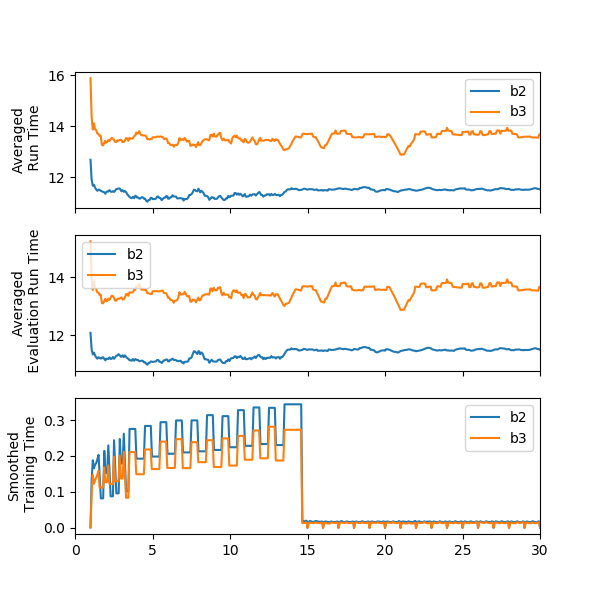
\includegraphics[width=.45\textwidth]{parts/appendix/reports-gmsnn/docs_esteban-latex/test_reports/2018-06-27/b2_b3_time.png} &
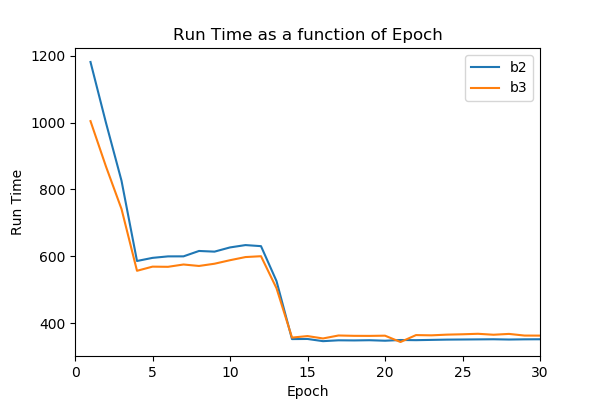
\includegraphics[width=.45\textwidth]{parts/appendix/reports-gmsnn/docs_esteban-latex/test_reports/2018-06-27/b2_b3_epoch.png} \tabularnewline

l & 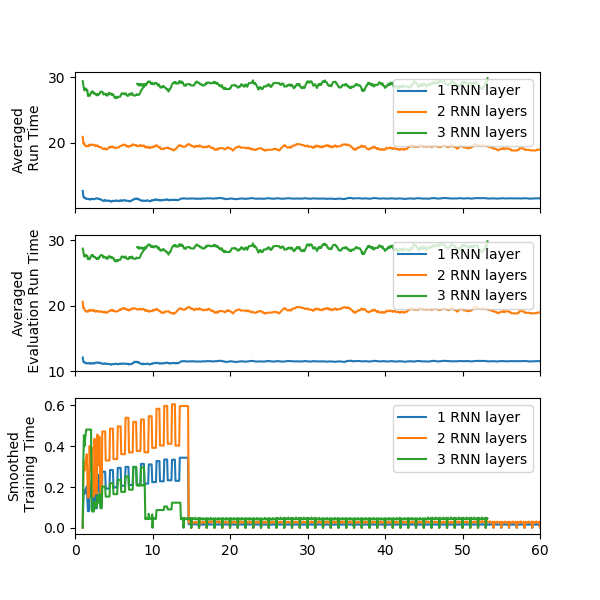
\includegraphics[width=.45\textwidth]{parts/appendix/reports-gmsnn/docs_esteban-latex/test_reports/2018-06-27/l_time.png} &
 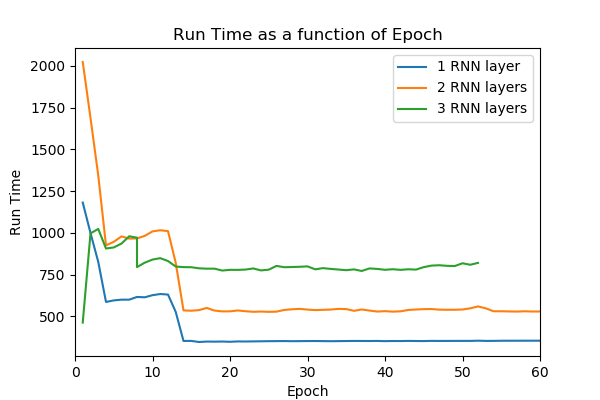
\includegraphics[width=.45\textwidth]{parts/appendix/reports-gmsnn/docs_esteban-latex/test_reports/2018-06-27/l_epoch.png} \tabularnewline

lbl & 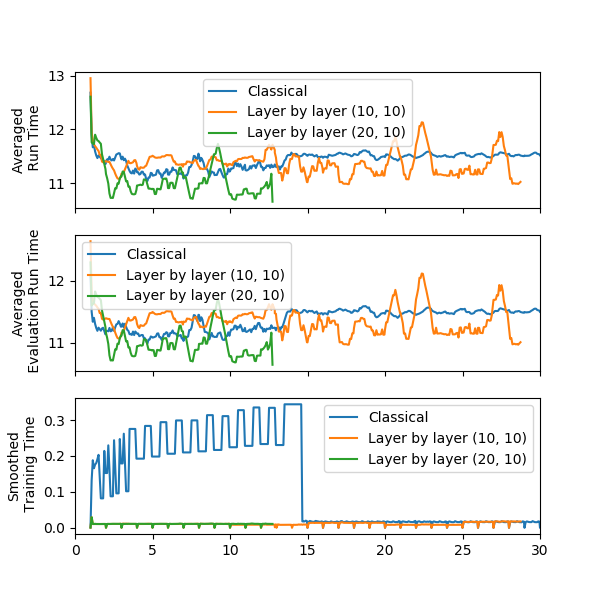
\includegraphics[width=.45\textwidth]{parts/appendix/reports-gmsnn/docs_esteban-latex/test_reports/2018-06-27/lbl_time.png} &
 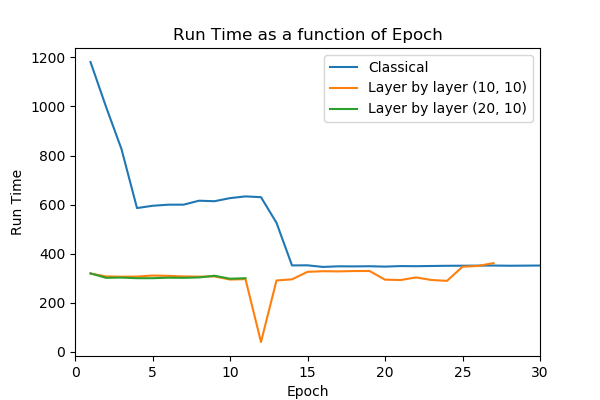
\includegraphics[width=.45\textwidth]{parts/appendix/reports-gmsnn/docs_esteban-latex/test_reports/2018-06-27/lbl_epoch.png} \tabularnewline

sum & 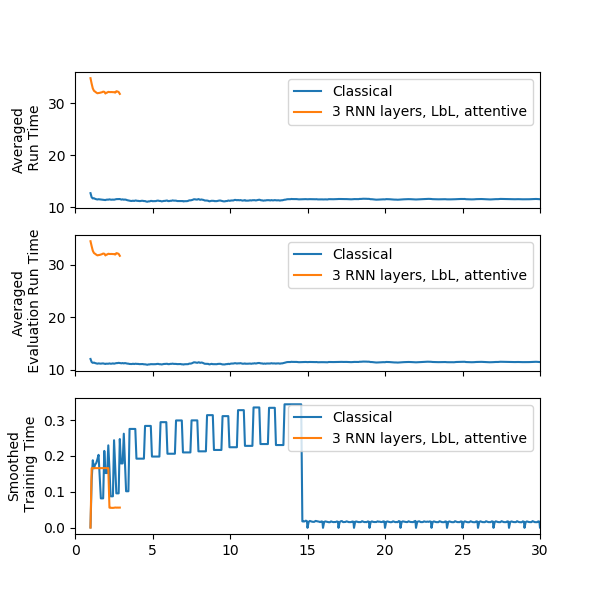
\includegraphics[width=.45\textwidth]{parts/appendix/reports-gmsnn/docs_esteban-latex/test_reports/2018-06-27/sum_time.png} &
 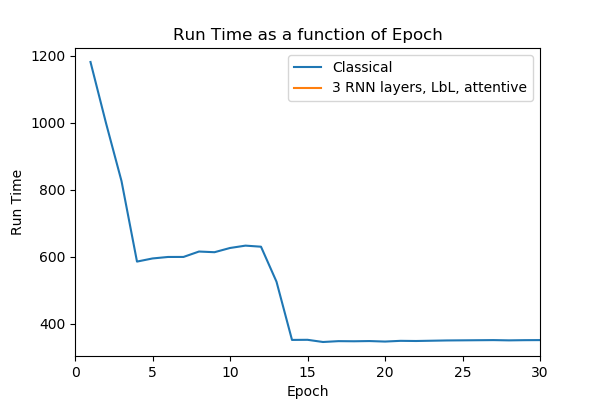
\includegraphics[width=.45\textwidth]{parts/appendix/reports-gmsnn/docs_esteban-latex/test_reports/2018-06-27/sum_epoch.png} \tabularnewline
\hline
\end{longtable}
\pagebreak
\begin{longtable}[]{@{}llll@{}}
\hline
Series & Memory & BPC & Full length
BPC\tabularnewline
\hline
\endhead
b2\_b3 & 
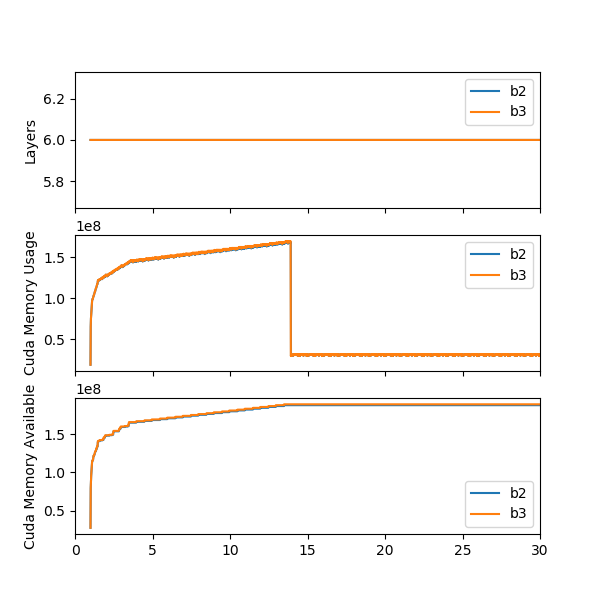
\includegraphics[width=.31\textwidth]{parts/appendix/reports-gmsnn/docs_esteban-latex/test_reports/2018-06-27/b2_b3_memory.png} &
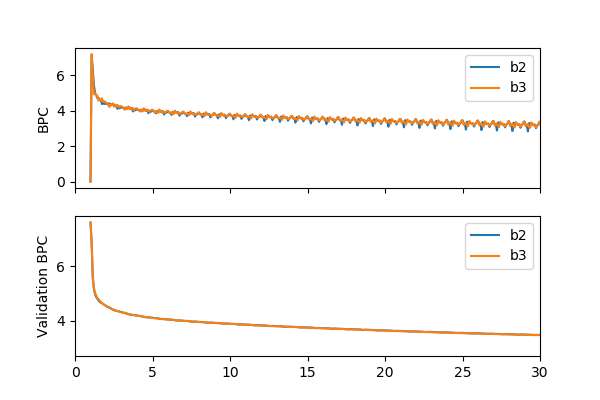
\includegraphics[width=.31\textwidth]{parts/appendix/reports-gmsnn/docs_esteban-latex/test_reports/2018-06-27/b2_b3_frac.png} &
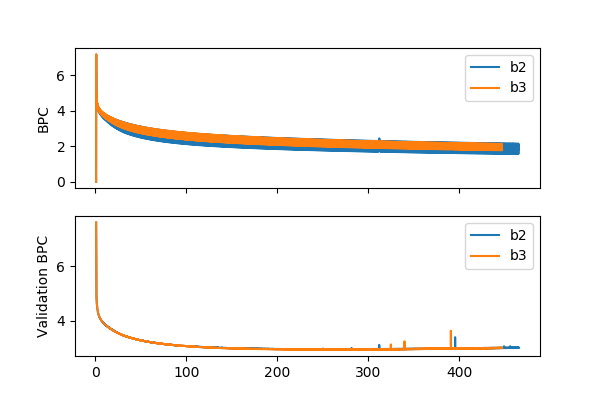
\includegraphics[width=.31\textwidth]{parts/appendix/reports-gmsnn/docs_esteban-latex/test_reports/2018-06-27/b2_b3_frac_full.png}\tabularnewline

l & 
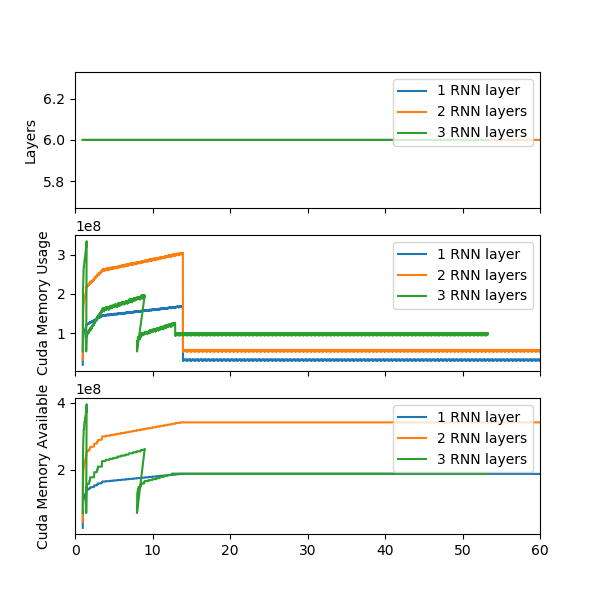
\includegraphics[width=.31\textwidth]{parts/appendix/reports-gmsnn/docs_esteban-latex/test_reports/2018-06-27/l_memory.png} &
 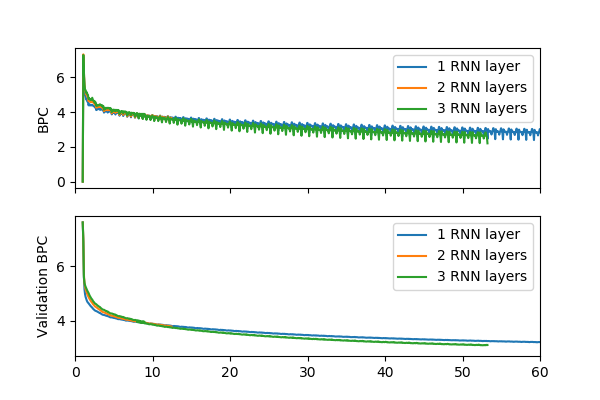
\includegraphics[width=.31\textwidth]{parts/appendix/reports-gmsnn/docs_esteban-latex/test_reports/2018-06-27/l_frac.png} &
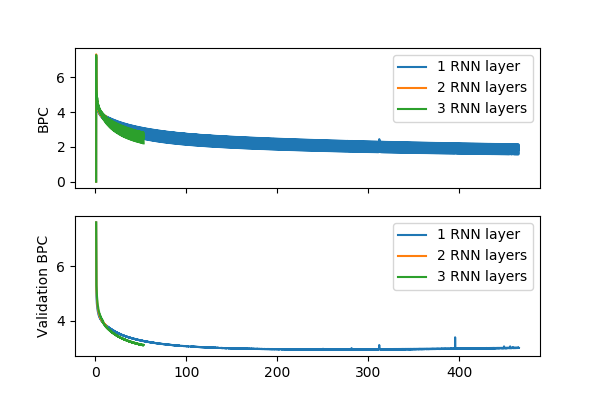
\includegraphics[width=.31\textwidth]{parts/appendix/reports-gmsnn/docs_esteban-latex/test_reports/2018-06-27/l_frac_full.png}\tabularnewline

lbl & 
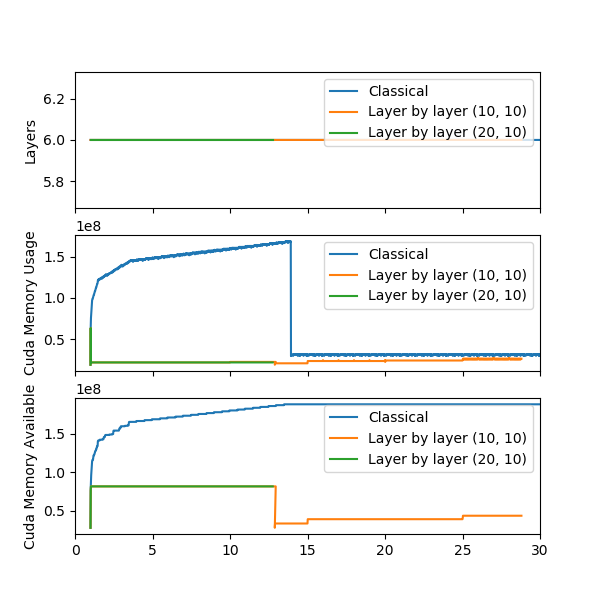
\includegraphics[width=.31\textwidth]{parts/appendix/reports-gmsnn/docs_esteban-latex/test_reports/2018-06-27/lbl_memory.png} & 
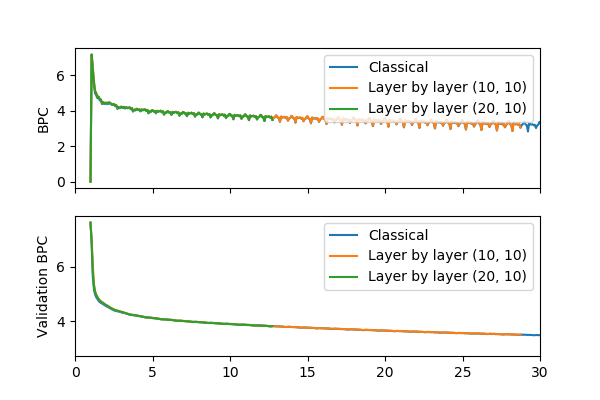
\includegraphics[width=.31\textwidth]{parts/appendix/reports-gmsnn/docs_esteban-latex/test_reports/2018-06-27/lbl_frac.png} &
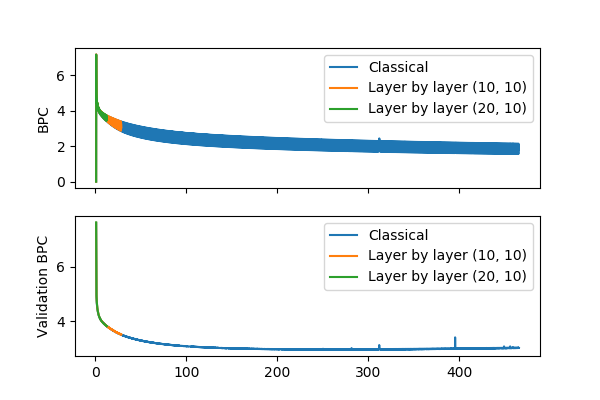
\includegraphics[width=.31\textwidth]{parts/appendix/reports-gmsnn/docs_esteban-latex/test_reports/2018-06-27/lbl_frac_full.png}\tabularnewline

sum & 
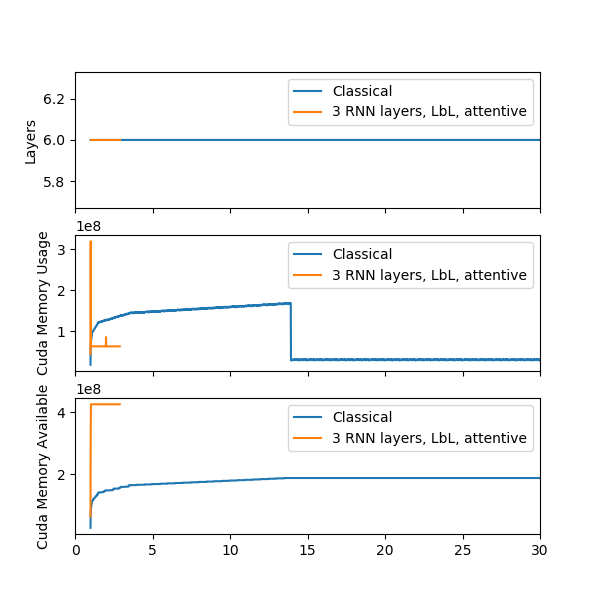
\includegraphics[width=.31\textwidth]{parts/appendix/reports-gmsnn/docs_esteban-latex/test_reports/2018-06-27/sum_memory.png} &
 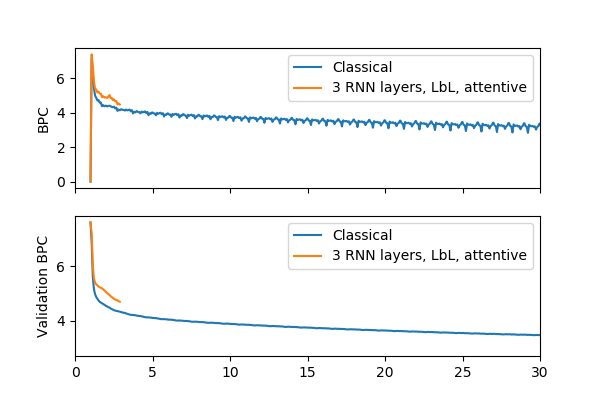
\includegraphics[width=.31\textwidth]{parts/appendix/reports-gmsnn/docs_esteban-latex/test_reports/2018-06-27/sum_frac.png} &
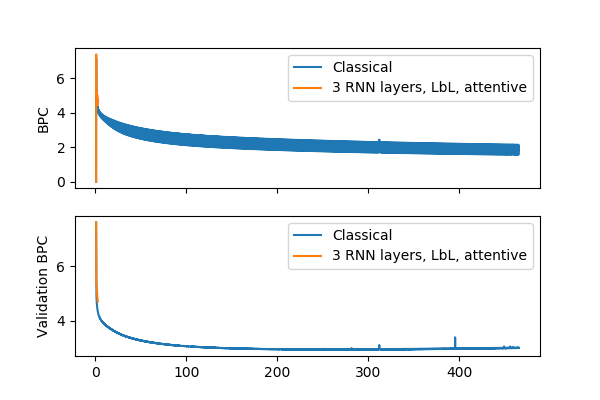
\includegraphics[width=.31\textwidth]{parts/appendix/reports-gmsnn/docs_esteban-latex/test_reports/2018-06-27/sum_frac_full.png}\tabularnewline
\hline
\end{longtable}

Plots will be referred to with : (Ex: ``l:Memory'')

\subsubsection{Time necessary to reach indicated validation
BPC}

\begin{longtable}[]{@{}lrrr@{}}
\hline
Model & 5 BPC & 4 BPC & 3 BPC\tabularnewline
\hline
\endhead
b2 & 0H 19M 41S & 1H 19M 47S & 15H 13M 7S\tabularnewline
b3 & 0H 16M 44S & 1H 11M 48S & 15H 3M 22S\tabularnewline
s & 0H 5M 19S & 0H 30M 59S &\tabularnewline
s-a20-l10 & 0H 5M 19S & 0H 30M 26S &\tabularnewline
l2 & 0H 33M 43S & 2H 27M 51S &\tabularnewline
l3 & \sout{0H 7M 41S} & \sout{2H 13M 2S} &\tabularnewline
s\_l3\_a & 0H 16M 7S & &\tabularnewline
\hline
\end{longtable}

Empty fields are where network has not reached BPC yet \sout{Crossed
out} fields are where data has been corrupted (because of an
interruption in training)

\subsubsection{Epochs necessary to reach indicated validation
BPC}

\begin{longtable}[]{@{}llll@{}}
\hline
Model & 5 BPC & 4 BPC & 3 BPC\tabularnewline
\hline
\endhead
b2 & 0.296 & 6.000 & 141.4\tabularnewline
b3 & 0.367 & 5.954 & 136.4\tabularnewline
s & 0.371 & 6.000 &\tabularnewline
s-a20-l10 & 0.371 & 6.000 &\tabularnewline
l2 & 0.593 & 6.519 &\tabularnewline
l3 & 0.816 & 7.296 &\tabularnewline
s\_l3\_a & 1.148 & &\tabularnewline
\hline
\end{longtable}

Empty fields are where network has not reached BPC yet

\subsection{Analysis}\label{analysis}

\subsubsection{\texorpdfstring{Run time and memory on ``l'' series
(l:memory, l:time, and l:time to run an
epoch)}{Run time and memory on l series (l:memory, l:time, and l:time to run an epoch)}}

Training of ``l3'' model was interrupted 2 times before the 15th epoch,
each time cleaning the memory, inducing training time reduction and
epoch time reduction (due to the correlation of memory usage and
training time).

\subsubsection{\texorpdfstring{Run time and memory on ``lbl'' series
(lbl:memory, lbl:time, and lbl:time to run an
epoch)}{Run time and memory on lbl series (lbl:memory, lbl:time, and lbl:time to run an epoch)}}

The specificity of layer by layer training are a lead to the cause of
the collapse of memory usage and run time during the 15th epoch.

During layer by layer training, memory usage is kept constant over the
first 15 epochs, whereas with classical training, memory usage increases
during ths period.

Layer by layer training reduces simultaneous graph accumulation over the
different epochs by training a layer at a time. It possibly reduces SGD
inertia too.

\subsubsection{Performance of layer by layer
training}

No notable variation on BPC. For run time and memory, see above.

\subsubsection{Performance of multi-RNN-layered
architecture}

A slight improvement of BPC can be seen with 3 layers (sadly, BPC data
for 2 layers is corrupted). Computation-time is proportional to the
number of layers (time data for 3 layers is unusable).

\subsubsection{Performance of 3 batches compared to 2
batches}

2 and 3 batches have an almost identical performance (time-wise,
BPC-wise and memory-wise), except 3 batches seem to get less dispersed
BPC.

\subsubsection{Results of long training with 2 and 3 batches
(b2\_b3:full length
bpc)}

The plot ``b2\_b3:full length bpc'' shows that after 200 epochs,
validation BPC stagnates. After 300 epochs, validation BPC begins to
increase very slowly, those are the first signs of over-fitting. These
observations were cross-checked with the raw data.

\subsubsection{Note on attention module}

A model with the attention module was tested for 5 hours, and did not
reach a full epoch. It can be deemed that without a training algorithm
like layer by layer training, using attention is not viable.
